 %volby: 
% male × female
% czech × english (zatím funguje jen czech)
% a studijní program / obor 
% is_bc (nejvíc odladěno)
% api_bc
% api_ing
% edu_bc
% edu_ing

\documentclass[male,czech,api_bc]{kitheses}
\usepackage{ifthen}

\usepackage{amsmath,amssymb}
\usepackage{graphics}
\usepackage{color}
\usepackage{array}
\usepackage{longtable}
\usepackage{afterpage}
\usepackage{microtype}  % přesnější typografie
\usepackage{tikz}
\usetikzlibrary{shapes.geometric, arrows.meta, positioning, fit, backgrounds}
\usepackage{float}

% workaround for imcompatibility of czech babel and biblatex

\iftutex
\else
\usepackage{etoolbox}
\makeatletter
\newcommand\my@hsyphen{-}
\newcommand\my@apostroph{'}
\patchcmd\select@language{-}{\my@hyphen }{}{\fail}
\patchcmd\select@language{'}{\my@apostroph }{}{\fail}
\makeatother
\fi

\usepackage[style=iso-numeric,shortnumeration=true]{biblatex}
\addbibresource{thesis.bib}


% fonty lze měnit (detaily viz sekce fonty)
\iftutex
	\usepackage{fontspec}  % nastavení fontů pro LuaLaTeX a XeLaTeX
	\setmainfont{Libertinus Serif}
	\setsansfont{Libertinus Sans}
	\setmonofont[Scale=MatchLowercase]{Source Code Pro}
	\usepackage{unicode-math}
	\setmathfont{Libertinus Math}
\else
	\usepackage[utf8]{inputenc} % nastavení pro PDF LaTeX
	\usepackage[T1]{fontenc}
	\usepackage{libertinus}
	\renewcommand{\ttdefault}{pxtt}
\fi

\usepackage{csquotes} % uvozovky

% sazba ukázek kódu 

\usepackage{listings}

% ukázka pro nastavení balíku listings pro sazbu ukázek zdrojových kódů
\lstset{ %
  language=Python,                % the language of the code
  basicstyle=\small\ttfamily,    
  backgroundcolor=\color{white},   % choose the background color. You must add \usepackage{color}
  showspaces=false,                % show spaces adding particular underscores
  showstringspaces=true,           % underline spaces within strings
  showtabs=false,                  % show tabs within strings adding particular underscores
  frame=single,                    % adds a frame around the code
  tabsize=3,                       % sets default tabsize to 2 spaces
  breaklines=true,                 % sets automatic line breaking
  breakatwhitespace=false,         % sets if automatic breaks should only happen at whitespace
  keywordstyle=\bfseries,          % keyword style
  commentstyle=\rmfamily,       % comment style
  stringstyle=\itshape\color,   % string literal style
}

% barevné zvýraznění textů, které je nutno nahradit
\newcommand{\ZT}[1]{\colorbox{yellow}{\color{red}{#1}}}


% TOTO JE POTŘEBA ZMĚNIT !!!!!!
\newcommand{\nazevcz}{Vylepšení bezpečnosti a správy uživatelských účtů na základní škole pomocí Azure Active Directory a Microsoft 365}     % zde VYPLŇTE český název práce (přesně podle zadání!)
\newcommand{\nazeven}{Improving Security and User Account Management at an Elementary School Using Azure Active Directory and Microsoft 365}   % zde VYPLŇTE anglický název práce (přesně podle zadání!)
\newcommand{\autor}{Bao Kieu Quang}          % zde VYPLŇTE své jméno a příjmení
\newcommand{\rok}{\the\year}                
\newcommand{\vedouci}{Ing. Pavel Kuba, Ph.D.}         
% zde VYPLŇTE jméno a příjmení vedoucího práce, včetně titulů
\newcommand{\vedouciDAT}{Ing. Pavlu Kubovi, Ph.D.}   
% zde VYPLŇTE jméno a příjmení vedoucího práce, včetně titulů ve třetím pádě
                                                           

% zvětšuje o 23% vertikální okraje v tabulkách
\renewcommand{\arraystretch}{1.23}

% nastavení pro záhlaví (co nelze udělat v cls souboru)

\renewcommand{\chaptermark}[1]{\markboth{\arabic{chapter}. #1}{}}
\pagestyle{fancy}

% nastavení odkazů
\usepackage{url} % formátování URL, příkaz \url
\usepackage{varioref} % lepší interní odkazy na obrázky, apod. příkaz \vref
\usepackage[unicode=true,pdfusetitle,
 bookmarks=true,
 breaklinks=false,pdfborder={0 0 1},backref=false,colorlinks=false]{hyperref} % hypertextové odkazy v PDF
 
\newcommand{\UV}[1]{\quotedblbase#1\textquotedblleft}
 
% odstraňte pokud vám vadí absence zarovnání dole 
\raggedbottom

%%%%%%%%%%%%%%%%%%%%%%%%%%%%%%%%%%%%%%%%%%%%%%
% vlastní začátek dokumentu
%%%%%%%%%%%%%%%%%%%%%%%%%%%%%%%%%%%%%%%%%%%%%%

\begin{document}
\thispagestyle{empty}
\begin{center}
{
\LARGE
\univerzita\\[16pt]
\fakulta
}

\vspace{2cm}
\resizebox{8.42cm}{!}{%
\ifthenelse{\boolean{czech}}
{
\includegraphics{LOGO_PRF_CZ_RGB_standard.jpg}}
{
\includegraphics{LOGO_PRF_EN_RGB_standard.jpg}}}

\vspace{2cm}
{
\Huge\sffamily
\nazevcz\par
\vspace{0.6cm}
\Large\scshape \ifthenelse{\boolean{bc}}{bakalářská}{diplomová} práce
}
\end{center} 
 
\vfill
{
\large
\begin{tabular}{>{\bfseries}rl}
    Vypracoval: 	& \autor\\
    Vedoucí práce: 	& \vedouci\\
&\\
Studijní program:       & \program\\

\end{tabular} 
}
\vspace{1.5cm}
\begin{center}
  \Large\scshape   Ústí nad Labem \rok
\end{center}

\cleardoublepage
\thispagestyle{empty}
\pagecolor{yellow}
{\Large Namísto žlutých stránek vložte digitálně podepsané zadání kvalifikační práce poskytnuté vedoucím katedry.\\\
Zadání musí zaujímat právě dvě strany.
}

Zadání je nutno vložit jako PDF pomocí některého nástroje, který umožňuje editaci dokumentů (se zachováním
elektronického podpisu).

V Linuxe lze například použít příkaz \texttt{pdftk}.

\clearpage
\thispagestyle{empty}
\afterpage{\nopagecolor}
~
\clearpage

\thispagestyle{empty} 
{\bfseries Prohlášení}

\vspace{0.5cm}
Prohlašuji, že jsem tuto \ifthenelse{\boolean{bc}}{bakalářskou}{diplomovou} práci vypracoval\ifthenelse{\boolean{feminum}}{a}{}
samostatně a použil\ifthenelse{\boolean{feminum}}{a}{}
jen pramenů, které cituji a uvádím v přiloženém seznamu literatury.

\vspace{0.5em}

Byl\ifthenelse{\boolean{feminum}}{a}{} jsem seznámen\ifthenelse{\boolean{feminum}}{a}{} 
s tím, že se na moji práci vztahují práva a povinnosti vyplývající ze
zákona č. 121/2000 Sb., ve znění zákona č. 81/2005 Sb., autorský zákon, zejména se
skutečností, že Univerzita Jana Evangelisty Purkyně v Ústí nad Labem má právo na uzavření
licenční smlouvy o užití této práce jako školního díla podle § 60 odst. 1 autorského zákona, a
s tím, že pokud dojde k užití této práce mnou nebo bude poskytnuta licence o užití jinému
subjektu, je Univerzita Jana Evangelisty Purkyně v Ústí nad Labem oprávněna ode mne
požadovat přiměřený příspěvek na úhradu nákladu, které na vytvoření díla vynaložila, a to
podle okolností až do jejich skutečné výše.

\vspace{2em}

V Ústí nad Labem dne \today   \hfill Podpis: \makebox[4cm][s]{\dotfill}

\cleardoublepage
\thispagestyle{empty}
~
\vfill

\begin{flushright}
    Děkuji vedoucímu práce {\vedouciDAT}\\
    za neocenitelné rady a pomoc při tvorbě bakalářské práce.
    
    Dále děkuji své rodině a nejbližším přátelům\\
    za podporu během studia a psaní závěrečné práce.
\end{flushright}

\cleardoublepage

\textsc{\nazevcz}

\textbf{Abstrakt:}

Digitalizace škol klade nové nároky na správu uživatelských identit a~kybernetickou bezpečnost. Školy se přitom často potýkají s~problémem sdílených lokálních účtů, které znemožňují dohledatelnost uživatelů a~jsou v~rozporu s~požadavky nařízení GDPR.
Pro ZŠ Vinařská bylo navrženo řešení postavené na přechodu na individuální cloudové identity spravované v~Microsoft Entra ID. Navržená architektura byla ověřena pilotním nasazením v~reálném prostředí školního tenanta Microsoft~365.
Výstupem práce je architekturní návrh správy identit a~skupin, nasazení vícefaktorového ověřování, podmíněného přístupu a~politik hesel, správa zařízení prostřednictvím Microsoft Intune včetně scénáře zapůjčeného notebooku a~implementační plán s~vyhodnocením přínosů a~rizik.
Pilotní nasazení potvrdilo funkčnost navrženého řešení a~tvoří základ pro plné produkční nasazení plánované na léto 2026.

\textbf{Klíčová slova:} kybernetická bezpečnost, správa identit, Microsoft Entra ID, Microsoft Intune, základní škola

\bigskip


\textsc{\nazeven}

\textbf{Abstract:}

The digitization of schools places new demands on user identity management and cybersecurity. Schools often face the problem of shared local accounts, which make it impossible to track users and violate GDPR requirements.
A solution was designed for Vinařská Elementary School based on a transition to individual cloud identities managed in Microsoft Entra ID. The proposed architecture was validated through a pilot deployment in a real-world Microsoft 365 school tenant environment.
The outputs of this work include an architectural design for identity and group management, the deployment of multi-factor authentication, conditional access, and password policies, device management via Microsoft Intune including a scenario for loaned laptops and an implementation plan with an assessment of benefits and risks.
The pilot deployment confirmed the functionality of the proposed solution and forms the basis for full production deployment planned for the summer of 2026.

\textbf{Keywords:} cybersecurity, identity management, Microsoft Entra ID, Microsoft Intune, elementary school

\tableofcontents

\addchap{Úvod}
Rostoucí digitalizace škol přináší nové požadavky na správu uživatelských 
identit a~zajištění kybernetické bezpečnosti. Školy dnes běžně využívají 
cloudové platformy pro výuku, komunikaci i~správu dat, přičemž bezpečnostní 
infrastruktura za tímto rozvojem často zaostává. Jedním z~nejrozšířenějších 
problémů je využívání sdílených lokálních účtů, které znemožňují přiřadit 
konkrétní činnost konkrétnímu uživateli, neumožňují vynucovat bezpečnostní 
politiky a~jsou v~rozporu s~požadavky nařízení GDPR na ochranu osobních 
údajů. Tento stav je typický zejména pro menší školy s~omezeným počtem 
IT pracovníků, kde bezpečnostní opatření ustupují provozní jednoduchosti.

Základní škola Vinařská v~Ústí nad Labem je konkrétním příkladem tohoto 
stavu. Škola v~rámci projektu Digitalizujeme školu získala licence 
Microsoft~365 Education~A3, které poskytují přístup k~nástrojům pro 
centrální správu identit a~zařízení. Přestože jsou tyto nástroje k~dispozici, 
nejsou dosud využívány, uživatelé se přihlašují ke cloudovým službám 
bez vícefaktorového ověřování, podmíněný přístup není nakonfigurován 
a~zařízení nejsou spravována centrálně. Tato práce vznikla v~přímé 
souvislosti s~působením autora jako IT administrátora školy a~vychází 
z~reálných poznatků o~stavu školní infrastruktury.

Hlavním cílem práce je navrhnout a~ověřit postup přechodu ze sdílených 
lokálních účtů na individuální cloudové identity spravované v~Microsoft 
Entra ID s~napojením na Microsoft~365 a~nasazením klíčových bezpečnostních 
politik. Dílčími cíli jsou návrh struktury identit a~skupin včetně 
standardu pojmenování, nasazení vícefaktorového ověřování a~podmíněného 
přístupu, zavedení správy zařízení prostřednictvím Microsoft Intune 
včetně scénáře zapůjčených notebooků a~vypracování implementačního plánu 
s~vyhodnocením přínosů a~rizik.

Teoretická část práce se věnuje specifikům školního IT prostředí, 
bezpečnostním politikám v~cloudu a~právním aspektům využití cloudových 
služeb ve školách. Praktická část analyzuje současný stav ZŠ Vinařská, 
navrhuje architekturu řešení a~dokumentuje pilotní nasazení provedené 
v~reálném prostředí školního tenanta Microsoft~365.

\chapter{Kybernetická bezpečnost a správa identit ve školním prostředí}

\section{Specifika školního IT prostředí}
Digitalizace škol klade nové nároky na IT infrastrukturu. Jedním z těchto nároků je vybudování bezpečného prostředí a zajištění vhodných podmínek na úrovni hardwaru, softwaru a infrastruktury potřebné pro jejich správu~\cite{DigitalizaceCR2025}.

Školy čelí specifickým výzvám, neboť pod jednou střechou sdružují velmi různorodou skupinu uživatelů, tedy děti i dospělé, osoby technicky zdatné i naprosté laiky. K tomu přistupuje vysoká fluktuace žáků, omezený počet IT pracovníků a povinnost chránit citlivé osobní údaje nezletilých. Právě v těchto ohledech se škola od běžné firmy zásadně liší a nelze na ni bez úprav aplikovat stejné přístupy ke kybernetické bezpečnosti~\cite{Benes2024}.

Důsledkem těchto omezení je, že v praxi se školy nezřídka uchylují ke kompromisním řešením. Jedním z nejrozšířenějších jsou sdílené uživatelské účty, které sice snižují nároky na správu, ale přinášejí nezanedbatelná bezpečnostní rizika. Udělení plného přístupu do systému žákovi či zaměstnanci bez jasně vymezených oprávnění může vést k narušení bezpečnosti a ohrožení ostatních uživatelů. Výjimku tvoří případy, kdy výuka sama o sobě rozšířená práva vyžaduje, i tehdy by však měla být udělena kontrolovaně a dočasně~\cite{AFCEA2024}.

Jako základ pro správné řešení NÚKIB\footnote{Národní úřad pro kybernetickou 
a informační bezpečnost — ústřední správní úřad České republiky odpovědný za 
kybernetickou bezpečnost.} ve spolupráci s AFCEA\footnote{Armed Forces 
Communications and Electronics Association — mezinárodní nezisková organizace 
sdružující odborníky z oblasti bezpečnosti, komunikací a informačních technologií.} 
doporučuje oddělení serverů, zařízení zaměstnanců, učebnových zařízení 
a soukromých zařízení žáků do samostatných segmentů. Toto rozdělení výrazně 
omezuje možný dopad případného bezpečnostního incidentu~\cite{AFCEA2024}.

Tato doporučení dále rozlišují dva typy bezpečnostních opatření: základní a rozšiřující. Základní opatření jsou závazná pro všechny školy a zahrnují řízení uživatelských oprávnění, zálohování, ochranu proti škodlivému kódu, patch management (správa aktualizací), logování a vzdělávání uživatelů. Rozšiřující opatření jsou dobrovolná, avšak doporučená pro zvýšení celkové úrovně zabezpečení, a zahrnují například content security management (správa obsahu) a základní bezpečnostní dohled~\cite{AFCEA2024}.

\section{Požadavky na kybernetickou bezpečnost}
Škola zpracovává citlivá data, a z toho vyplývají konkrétní povinnosti jako je GDPR (General Data Protection Regulation), jež ukládá školám povinnost chránit osobní údaje, a to zejména údaje nezletilých~\cite{GDPR2016}. Bezpečnostní politiky musí být nastaveny tak, aby byly jasné a srozumitelné pro žáky i učitele v souladu s GDPR a pravidelně zapojovat všechny skupiny (vedení, IT, učitele, žáky, rodiče). Technická opatření jako taková nestačí, je nutná metodika a školení~\cite{Benes2024}.

Správce IT nese etickou odpovědnost za nakládání s daty nezletilých a musí systém nastavit tak, aby minimalizoval riziko pro uživatele, kteří sami nemohou posoudit důsledky sdílení svých dat. Tato odpovědnost přesahuje právní povinnost, jde o aktivní ochranu, nikoliv jen splnění formálních požadavků~\cite{Benes2024, AFCEA2024}.

Vedle organizačních požadavků je důležité ukotvit i technické principy bezpečnosti. Ve školním prostředí by se měla aplikovat CIA triáda (Confidentiality, Integrity, Availability), tedy tři základní pilíře informační bezpečnosti: důvěrnost, integrita a dostupnost. V kontextu školy to znamená konkrétní požadavky. Důvěrnost chrání osobní údaje žáků před neoprávněným přístupem, což je obzvláště důležité s ohledem na zpracování dat nezletilých. Integrita zaručuje, že studijní výsledky či docházka nebudou neoprávněně pozměněny. Dostupnost pak zajišťuje, že učitelé i žáci mají přístup k potřebným systémům v době výuky~\cite{Benes2024}.

\section{Microsoft 365 pro vzdělávání a Microsoft Entra ID}
Microsoft 365 (dále jen M365) jako cloudová služba odpovídá na problémy škol. Ve vzdělání se mezi žáky a učiteli využívají komunikační a kancelářské nástroje. Tento ekosystém však nabízí výrazně více, zejména na úrovni správy identit a kybernetické bezpečnosti~\cite{Office365_article}.

Microsoft nabízí tři varianty licencí, které lze využít ve vzdělaní, A1, A3 a A5. Licence A1 je základní variantou, která pokrývá základní kancelářské a komunikační nástroje. A3 přidává Intune a Entra ID, které jsou klíčovými nástroje při správě zařízení a identit. A5 pak rozšiřuje nabídku o pokročilou bezpečnostní analytiku a ochranu před hrozbami (threat protection). Pro školy, které usilují o zavedení centrální správy identit a zařízení, představuje licence A3 dostačující základ bez nutnosti investice do nejvyšší varianty~\cite{MicrosoftM365Edu2025}.

Microsoft Entra ID je cloudovou alternativou pro tradiční lokálně provozovanou adresářovou službu (on-premise Active Directory). Základní funkce, kterými disponuje, jsou správa uživatelů, skupin, rolí a jednotné přihlášení (SSO, z angl. Single Sign-On). Pojem SSO znamená, že se uživatel přihlásí jednou a má přístup ke všem propojeným službám, například se učitel přihlásí jednou a má přístup do Teams, SharePointu i k dalším službám bez opakovaného zadávání hesla~\cite{MicrosoftEntra2025}.

V rámci Entra ID jsou klíčové funkce jako vícefaktorové ověřování (MFA, z angl. Multi-Factor Authentication), která slouží jako vrstva ochrany nad heslem. Podmíněný přístup (Conditional Access) představuje mechanismus, který definuje za jakých podmínek přístup povolí nebo zamítne, například ze zařízení zaregistrovaného v Intune, jehož role je podrobněji popsána v následující kapitole. Vzhledem k již zmíněné vysoké fluktuaci uživatelů právě kombinace těchto nástrojů umožňuje efektivní správu v tomto prostředí~\cite{EntraID_article}. Konkrétní konfigurace těchto bezpečnostních mechanismů a jejich nasazení v prostředí školy je předmětem následující kapitoly.

\chapter{Bezpečnostní politiky a správa zařízení v cloudu}
Samotný účet s heslem je jen první linie. Heslo může být prolomeno, uhádnuto nebo ukradnuto a to platí dvojnásob ve školním prostředí, kde uživatelé nejsou bezpečnostně školeni. Proto se nad správou identit přidávají další vrstvy jako je MFA, podmíněný přístup a Intune. Každá vrstva staví na té předchozí, přičemž MFA ověří identitu, dále podmíněný přístup rozhodne za jakých podmínek přístup povolí, Intune zajistí, že samotné zařízení splňuje bezpečnostní požadavky.

\section{Vícefaktorové ověřování (MFA)}
Hesla se dnes opakují napříč službami, uživatelé volí slabá hesla, tudíž je kompromitace hesla reálná hrozba. Vícefaktorové ověřování zajišťuje, že i při kompromitaci hesla útočník přístup nezíská.

Princip MFA má tři kategorie faktorů nimiž jsou znalost, držení a vlastnost. Znalost značí něco co víme, tím se značí například heslo, PIN kód nebo odpověď na bezpečnostní otázku. Kategorie držení zahrnuje předměty v fyzické držbě uživatele, tedy například mobilní telefon, čipovou kartu nebo hardwarový token. Kategorie vlastnosti zahrnuje biometrické charakteristiky uživatele, jako jsou například otisk prstu, sken obličeje nebo oční duhovky~\cite{NIST_SP800634}.

Metod pro ověřování je vícero a mohou se lišit na úrovni zabezpečení a jakým útokům mohou čelit. Mezi nejméně bezpečné patří SMS nebo e-mail, a to právě kvůli jejich náchylnosti na zachycení a SIM swapping, tedy útok, při kterém útočník přesměruje telefonní číslo oběti na vlastní SIM kartu a tím získá přístup k ověřovacím SMS zprávám. Autentizační aplikace jako Microsoft/Google Authenticator nabízejí vyšší bezpečnost pomocí jednorázových či časově omezených kódů nebo nabízených oznámení (push notifikací), které mohou být zneužity při útoku zvaném zahlcení MFA výzvami (MFA fatigue), kdy útočník opakovaně odesílá ověřovací notifikace a spoléhá na to, že je uživatel omylem potvrdí. Nejvyšší úroveň ochrany dnes zajišťuje FIDO2 (Fast Identity Online 2), standard pro bezheslové ověřování pomocí hardwarových klíčů nebo biometrie, který je zároveň uživatelsky přívětivý~\cite{MicrosoftFIDO2,MicrosoftEntra2025}.

Volba metody MFA se liší podle skupiny uživatelů. Správci potřebují nejsilnější metody, učitelé silné, ale použitelné a žáci budou mít specifické omezení, každý nemusí mít vlastní telefon pro ověřování.

\section{Politiky hesel a podmíněný přístup}
Silná politika hesel je tvořena souborem pravidel, které definují požadavky pro tvorbu a správu hesla. Staré metody jako pravidelné nucené změny hesla a složité požadavky na speciální znaky selhávaly, protože uživatelé jsou předvídatelní přičemž obměna jediného znaku splňovala požadavky politiky u hesla. Moderní pohled od NISTu (Národní institut standardů a technologie) a Microsoftu prosazuje upřednostnění délky hesla před složitostí, blokování kompromitovaných hesel a politiku blokování účtu (lockout)~\cite{NIST_SP800634}. Silná politika hesel tak tvoří první vrstvu zabezpečení, avšak sama o~sobě nestačí. Podmíněný přístup proto přidává další úroveň ochrany, která rozhoduje na základě kontextových signálů, jako je lokalita, zařízení nebo rizikovost přihlášení.

Podmíněný přístup vyhodnocuje sadu signálů a na jejich základě rozhoduje o způsobu ověření uživatele. Systém poté může hned udělit přístup, zamítnout ho nebo si vyžádat MFA. Podmínek pro toto rozhodnutí je vícero, například uživatel/skupina, lokalita, zařízení splňující požadavky zásad (compliant device) spravované přes Intune a rizikovost přihlášení. Lokalita může být definována například jako důvěryhodná školní síť, přičemž přihlášení mimo ni může vyžadovat dodatečné ověření~\cite{MicrosoftEntra2025}.

\section{Microsoft Intune}
Správa zařízení v prostředí, kde uživatelé přistupují k citlivým datům vyžaduje centralizovaný nástroj. Microsoft Intune je cloudová služba, která spravuje uživatelská zařízení v rámci infrastruktury. Intune nabízí dva režimy spravování, MDM (Mobile Device Management) spravující celé zařízení a MAM (Mobile Application Management) spravující pouze aplikace. MDM je vhodné pro zařízení vlastněná organizací, MAM pro osobní zařízení uživatelů~\cite{MicrosoftIntune2025}.

Zařízení lze do infrastruktury zapojit například plně cloudově bez lokálního Active Directory (dále jen AD) přes Entra ID Join nebo kombinace s lokálním AD. Pro školy bez lokálního AD je Entra ID přirozenou volbou, protože nevyžaduje lokální infrastrukturu a vše je řízeno z cloudu přes Intune~\cite{MicrosoftIntune2025}.

Zařízení připojená do AD mají nastavené konfigurační profily, které nastavují omezení, proxy a BitLocker, tedy nástroj pro šifrování disku zabudovaný ve Windows, jenž chrání data v případě ztráty nebo krádeže zařízení. Vedle konfiguračních profilů existuje politika dodržování požadavků, která hodnotí zda jsou požadavky splněny. Rozdíl spočívá v tom, že konfigurační profil aktivně nastavuje parametry, zatímco politika dodržování požadavků pouze ověřuje jejich splnění. Podmíněný přístup tento stav následně využívá jako jeden ze signálů při rozhodování o~přístupu uživatele~\cite{MicrosoftIntune2025}.

Vzdálená správa dovoluje provádět například vzdálené vymazání (remote wipe) a selektivní vymazání (selective wipe), což je důležité pro zařízení zapůjčená žákům k domácímu použití. Vzdálené vymazání smaže celý přístroj a vrátí ho do továrního nastavení, používá se při ztrátě nebo krádeži zařízení, nebo při vyřazení z organizace. Selektivní vymazání smaže pouze firemní data a aplikace, osobní data zůstanou nedotčena. Používá se hlavně v MAM režimu, kdy uživatel používá vlastní koncové zařízení. Životní cyklus zařízení v Intune zahrnuje celou cestu od registrace zařízení přes konfiguraci a údržbu až po jeho vyřazení. Součástí je centralizovaná správa aktualizací operačního systému a aplikací~\cite{MicrosoftIntune2025}.

\chapter{Právní, etické a ekonomické aspekty cloudových služeb ve školách}
Škola nemusí řešit pouze to, jak zapojí vše v infrastruktuře, musí i vědět, jak nakládat s daty zpracovávanými v rámci této infrastruktury. Musí se přitom řídit určitými pravidly, která stanovují, jak s daty zacházet. Využívá k tomu dostupné technické prostředky a tím spravuje a chrání data, avšak tyto prostředky s sebou nesou provozní náklady. Z těchto důvodů se kapitola věnuje právní (GDPR), smluvní (licence) a ekonomické rovině. 

\section{GDPR a ochrana osobních údajů}
Jak bylo nastíněno v~kapitole~1.2, škola má z~nařízení GDPR konkrétní povinnosti, které se v~cloudovém prostředí projevují zejména v~oblasti vymezení rolí správce a zpracovatele dat.
Škola jakožto správce rozhoduje o účelu a prostředcích zpracování osobních údajů, což je definující povinnost dle nařízení GDPR. Microsoft jako zpracovatel nakládá s daty na základě pokynů správce, nikoliv samostatně. Ačkoliv se jedná o dvě rozdílné role, je třeba jejich vzájemný smluvní vztah formalizovat, což vede k uzavření zpracovatelské smlouvy (DPA)~\cite{GDPR2016}.

Dodatek o ochraně osobních údajů (Data Protection Addendum, DPA) je smlouva o zpracování osobních údajů pro vzdělávací instituce dle nařízení GDPR, jedná se o povinný doklad mezi správcem a zpracovatelem. Škola vystupuje jako správce, Microsoft jako zpracovatel a GDPR vyžaduje, aby zpracovatel poskytl správci dostatečné záruky splnění klíčových požadavků nařízení. DPA definuje podmínky, účel, jaká data jsou evidována, kde jsou uložena a za jakých podmínek mohou být předána třetím stranám. Škola ho nepodepisuje samostatně, ale přijímá jeho podmínky automaticky uzavřením smlouvy na služby M365. Data jsou uložena výhradně v rámci tzv. EU Data Boundary, tedy závazek Microsoftu uchovávat a zpracovávat data zákazníků z EU výhradně v datových centrech uvnitř Evropské unie~\cite{MicrosoftDPA2025}.

GDPR rozlišuje různé právní základy pro nakládání s osobními údaji a souhlas je jedním z nich. Škola může nakládat s daty žáků i bez souhlasu, pokud tato činnost vyplývá z jejích zákonných povinností (např. vedení třídní knihy) nebo oprávněného zájmu. Souhlas je potřeba až tehdy, kdy tato činnost přesahuje uvedený rámec. V kontextu M365 to znamená, že vytvoření školního účtu žáka je zpravidla zákonná povinnost nebo oprávněný zájem školy, tudíž souhlas není nutný. Nakládání s daty v cloudové službě třetí strany však může být citlivější, škola by proto měla mít jasno, jaká data jsou předávána do cloudové služby a na jakém právním základě. Souhlas bude vyžadován v případě, kdy rozsah nakládání s daty přesahuje rámec provozu služby, například při využití marketingových funkcí~\cite{GDPR2016, MicrosoftDPA2025}.

Škola dle GDPR musí vést záznam o všech činnostech nakládání s osobními údaji. Tento dokument není pouhou formalitou, jde o dokument, který škola předloží dozorovému úřadu při kontrole. Záznam obsahuje účely vedení dat, kategorie subjektů a dat, příjemce včetně zpracovatelů a lhůty výmazu. V kontextu M365 to znamená, že škola musí mít v záznamu explicitně uvedeno, že Microsoft je příjemcem dat žáků a učitelů jako smluvní zpracovatel na základě uzavřeného DPA~\cite{GDPR2016}.

Při výběru cloudové služby je rovněž vhodné zohlednit bezpečnostní 
klasifikaci poskytovatele. NÚKIB vydal průvodce zařazením cloud computingu 
do bezpečnostních úrovní, který definuje požadavky na poskytovatele 
v~závislosti na citlivosti zpracovávaných dat~\cite{NUKIB2023}.

\section{Licenční a smluvní aspekty}
Volba licence je zásadní rozhodnutí, které má přímý dopad na to, jaké bezpečnostní nástroje má škola k dispozici. A1 je bezplatná varianta dostupná způsobilým vzdělávacím institucím. Poskytuje webové verze Office aplikací a základní nástroje pro spolupráci jako Teams, OneDrive a SharePoint. A3 rozšiřuje A1 o bezpečnostní nástroje a pokročilou správu zařízení. A3 zahrnuje desktopové verze Office aplikací, Microsoft Intune pro správu zařízení a Entra ID Premium P1, který umožňuje nasazení podmíněného přístupu (Conditional Access) a vícefaktorového ověřování (MFA). Smluvní podmínky škola přijímá automaticky při aktivaci služby, nikoliv samostatným podpisem smlouvy~\cite{MicrosoftM365Edu2025}.

Škola přijímá dva dokumenty, Product Terms (smluvní podmínky produktů) a DPA, které společně tvoří celý smluvní rámec. Microsoft může podmínky aktualizovat, tudíž by škola měla jejich změny sledovat, zejména u DPA, kde změny mohou mít dopad na ochranu osobních údajů žáků. Škola nemá prostor podmínky vyjednávat a přijímá je jako celek, což je standardní model cloudových služeb~\cite{MicrosoftDPA2025}.

\section{Ekonomické aspekty}
Při výběru cloudové služby nestačí porovnat ceny, je nutné zohlednit celkové náklady na vlastnictví, dostupné alternativy a dlouhodobou provozní udržitelnost.

Celkové náklady na vlastnictví (TCO, z angl. Total Cost of Ownership) vyjadřuje celkové náklady na vlastnictví a provoz řešení. Zahrnuje počáteční investici, pravidelné výdaje a výdaje při ukončení. Cloudové řešení snižuje TCO oproti on-premise řešení, protože odpadají výdaje na hardware, servery, elektřinu a údržbu. Nákladem však zůstává čas správce při implementaci a školení uživatelů, což jsou reálné výdaje i u cloudového řešení~\cite{Nayar2018}.

Základní alternativou ke cloudovému řešení je on-premise přístup, tedy provoz vlastního serveru. Poskytuje plnou kontrolu bez závislosti na cloudovém poskytovateli. Naopak s sebou nese vysoké pořizovací výdaje, nutnost zajistit fyzickou bezpečnost, zálohy a aktualizace, což je pro malou školu s jedním IT správcem prakticky neudržitelné~\cite{Nayar2018}. Možností by byl také Google Workspace for Education, který je také zdarma pro školy, obsahuje Gmail, Drive, Meet a Classroom, ale chybí Intune, Conditional Access a Entra ID. Škola již M365 a licence A3 aktivně využívá, tudíž přechod na jinou platformu by znamenal ztrátu stávající konfigurace a investic~\cite{MicrosoftM365Edu2025}.

Provoz platformy závisí na interním správci, přičemž jeho případný odchod představuje riziko pro kontinuitu správy. M365 toto riziko částečně snižuje tím, že administrace je intuitivní a dobře dokumentovaná. Škola navíc není zcela závislá na interním správci, neboť A3 licence zahrnuje technickou podporu, přičemž dlouhodobá udržitelnost závisí i na důsledném používání platformy ze strany učitelů a žáků. Cloud se aktualizuje automaticky, škola tedy nemusí řešit upgrady jako u on-premise~\cite{MicrosoftM365Edu2025, Nayar2018}.

\chapter{Analýza současného stavu a návrh řešení}

\section{Charakteristika školy}

Základní škola Vinařská (dále jen „ZŠ Vinařská") je příspěvková organizace 
zřízená Statutárním městem Ústí nad Labem. Škola poskytuje základní vzdělání v~ročnících prvního a~druhého stupně, přičemž součástí organizace je rovněž přípravný ročník. Kapacita školy činí 387~žáků, v~době zpracování této práce školu reálně navštěvuje přibližně 300~žáků. Pedagogický sbor tvoří přibližně 40~učitelů, celkový počet zaměstnanců zahrnuje rovněž nepedagogické a~administrativní pracovníky. Škola se profiluje jako sportovní, součástí nabídky jsou třídy s~rozšířenou výukou tělesné výchovy zaměřené na lední hokej a~roztleskávačky.

Správu IT infrastruktury zajišťuje IT administrátor zodpovědný za provoz 
a~údržbu veškerého hardwaru, softwarového vybavení i~cloudových služeb. 
Škola disponuje počítačovou učebnou s~25~stolními počítači určenými primárně 
pro výuku a~dále přibližně 40~přenosnými počítači, 18~kusů ve sborovně a~22~kusů v~učebně fyziky. 
Zařízení jsou určena především pro výuku žáků v~případech, kdy není dostupná počítačová učebna nebo kdy pedagog preferuje mobilní řešení přímo ve třídě. 
Zapůjčení probíhá na vyžádání prostřednictvím sekretariátu nebo kabinetu fyziky, přičemž zařízení mohou využívat i~učitelé, kteří nemají přidělený vlastní pracovní notebook. 
K~dispozici je rovněž administrativní počítač pro potřeby 
vedení školy. Pro lokální sdílení souborů v~rámci školní sítě je provozován 
server NAS (Network Attached Storage), škola jinak nedisponuje vlastní 
serverovou infrastrukturou ani lokální adresářovou službou.

V~oblasti cloudových služeb využívá škola platformu Microsoft~365 Education, 
do níž se zapojila prostřednictvím projektu \textit{Digitalizujeme školu}. Na základě 
přidělených licencí typu A3 disponují všichni zaměstnanci i~žáci školními 
\mbox{e-mailovými} účty a~přístupem k~aplikacím sady Microsoft~365. V~praxi je však 
využití těchto nástrojů nerovnoměrné. Komunikační platforma Microsoft Teams 
a~\mbox{e--mailová} služba Exchange Online jsou využívány především pedagogickými 
pracovníky, přičemž míra zapojení se mezi jednotlivými učiteli liší. Žáci 
mají účty zřízeny, avšak jejich reálné využití cloudových služeb je minimální. 
Ostatní nástroje sady, jako jsou SharePoint nebo OneDrive, nejsou na úrovni 
školy systematicky zavedeny.

\section{Analýza současného stavu}

Současný stav správy identit a~přístupu na ZŠ Vinařská odráží situaci typickou 
pro školy, které postupně přecházejí z~tradičního lokálního prostředí do cloudu, 
avšak bez souběžného zavedení odpovídajících bezpečnostních opatření. Analýza 
vychází z~poznatků získaných při správě školní IT infrastruktury.

\subsection{Správa lokálních účtů}

Počítače v~učebně informatiky jsou provozovány jako samostatné stanice bez 
připojení k~doméně ani k~jinému centrálnímu adresářovému systému. Na každém 
zařízení jsou zřízeny dva lokální účty: účet s~administrátorskými oprávněními 
a~účet určený pro běžnou práci žáků. Hesla obou účtů jsou na všech počítačích 
totožná a~spravována centrálně IT administrátorem.

Tento přístup s sebou nese několik zásadních bezpečnostních rizik. Sdílené 
přihlašovací údaje znemožňují přiřadit konkrétní činnost konkrétnímu uživateli, 
čímž zcela chybí auditní stopa. V~případě bezpečnostního incidentu nelze 
zpětně zjistit, který žák nebo uživatel danou akci provedl. Dalším rizikem 
je skutečnost, že znalost hesla se mezi žáky může šířit nekontrolovatelně, čímž 
se zvyšuje pravděpodobnost zneužití. Přítomnost účtu s~administrátorskými 
oprávněními se sdíleným heslem pak představuje obzvláště závažné riziko, 
neboť případný útočník nebo i~samotný žák může získat plnou kontrolu nad zařízením.

Notebooky přidělené učitelům jsou oproti tomu vybaveny individuálními lokálními 
účty. Každý pedagog má vlastní přihlašovací údaje, což umožňuje základní 
oddělení uživatelských prostředí. Ani tato zařízení však nejsou součástí 
centrálně spravované infrastruktury a~nelze proto vynucovat jednotné 
bezpečnostní politiky, jako jsou požadavky na složitost hesla, automatické 
zamykání obrazovky, nebo šifrování disku.

\subsection{Správa cloudových identit}

V~rámci platformy Microsoft~365 Education je v~tenantovi (cloudovém prostředí organizace v rámci Microsoft 365) školy evidováno 
321~uživatelských účtů zahrnujících žáky, pedagogy a~administrativní 
pracovníky. Účty jsou zřizovány a~spravovány IT administrátorem, žáci 
ani jejich zákonní zástupci nemají možnost samostatně provádět změny 
přihlašovacích údajů.

Z~hlediska vícefaktorového ověřování je situace kritická, zejména pro administrátory a pedagogy. V~době zpracování 
této práce jsou v~tenantovi deaktivovány všechny standardní metody 
vícefaktorového ověřování, včetně aplikace Microsoft Authenticator, 
ověření prostřednictvím SMS a~hardwarových klíčů FIDO2. Jedinou aktivní 
metodou ověřování je jednorázový kód zasílaný e-mailem (Email One-Time 
Passcode, OTP). Tato metoda neposkytuje dostatečnou ochranu, neboť nevyžaduje 
prokázání držení druhého faktoru odděleného od primárního přihlašovacího 
kanálu a~je náchylná na phishingové útoky.
Pro žáky základní školy není nasazení vícefaktorového ověřování reálné, neboť ne každý žák disponuje vlastním zařízením potřebným pro ověřování.

Podmíněný přístup (Conditional Access) není nakonfigurován. Uživatelé se 
tedy mohou přihlašovat ke cloudovým službám školy z~libovolného zařízení 
a~z~libovolné sítě bez jakéhokoli omezení. Neexistuje rovněž žádný mechanismus, 
který by vyhodnocoval rizikové přihlášení, například pokus o~přihlášení 
z~neobvyklé geografické polohy nebo z~neznámého zařízení.

\subsection{Dopady na ochranu osobních údajů}

Popsaný stav má přímé dopady na plnění povinností vyplývajících z~nařízení 
GDPR. Sdílené lokální účty v~učebně znemožňují přiřadit zpracování osobních 
údajů konkrétní fyzické osobě, což je v~rozporu se zásadou odpovědnosti 
a~prokazatelnosti stanovenou v~článku~5 odst.~2 nařízení GDPR \cite{GDPR2016}. 
Absence auditních záznamů dále znamená, že škola není schopna doložit, kdo 
a~kdy s~osobními údaji pracoval, ani prokázat, že nedošlo k~neoprávněnému 
přístupu.

Absence vícefaktorového ověřování u~cloudových účtů zvyšuje riziko 
neoprávněného přístupu k~datům uloženým v~prostředí Microsoft~365, 
která mohou zahrnovat osobní údaje žáků i~zaměstnanců. Škola má přitom 
v~rámci GDPR povinnost přijmout vhodná technická a~organizační opatření 
zajišťující odpovídající úroveň zabezpečení osobních údajů, jak vyžaduje 
článek~32 téhož nařízení \cite{GDPR2016}.

\begin{table}[h]
\centering
\caption{Přehled zjištěných nedostatků v~oblasti správy identit a~přístupu}
\label{tab:nedostatky}
\begin{tabular}{|p{3.5cm}|p{5cm}|p{5cm}|}
\hline
\textbf{Oblast} & \textbf{Současný stav} & \textbf{Riziko} \\
\hline
Přihlášení žáků v~učebně & 
Sdílené lokální účty se stejným heslem na všech stanicích & 
Nelze přiřadit činnost konkrétnímu uživateli, chybí auditní stopa \\
\hline
Administrátorský účet & 
Sdílené heslo k~účtu s~plnými oprávněními & 
Možnost získání plné kontroly nad zařízením neoprávněnou osobou \\
\hline
Správa učitelských zařízení & 
Individuální lokální účty bez centrální správy & 
Nelze vynucovat bezpečnostní politiky (hesla, šifrování, zamykání) \\
\hline
Připojení zařízení & 
Standalone stanice bez domény ani adresářové služby & 
Žádná centrální viditelnost ani kontrola nad zařízeními \\
\hline
Vícefaktorové ověřování & 
Deaktivováno; aktivní pouze Email OTP & 
Zvýšené riziko kompromitace cloudových účtů \\
\hline
Podmíněný přístup & 
Není nakonfigurován & 
Přihlášení možné z~libovolného zařízení a~sítě bez omezení \\
\hline
Auditní záznamy & 
Neprobíhá žádné logování přihlášení ani aktivit & 
Nelze dohledat původce incidentu ani prokázat soulad s~GDPR \\
\hline
\end{tabular}
\end{table}

Zjištěné nedostatky tak vytvářejí konkrétní a~bezprostřední potřebu 
implementovat systém individuálních cloudových identit doplněný o~odpovídající 
bezpečnostní mechanismy, což je předmětem návrhu řešení popsaného 
v~následující části.

\section{Návrh architektury správy identit}

Na základě zjištěných nedostatků popsaných v~předchozí části je navrženo řešení 
postavené na centrální správě cloudových identit prostřednictvím platformy 
Microsoft Entra ID. Cílem návrhu je přechod od sdílených lokálních účtů 
k~individuálním cloudovým identitám, zavedení vícefaktorového ověřování pro 
privilegované uživatele a~připojení vybraných zařízení do cloudové adresářové 
služby. Vzhledem k~provozním omezením školy, zejména probíhajícímu školnímu 
roku a~skutečnosti, že část zařízení je provozována v~rámci pronájmu od 
externího poskytovatele, nebude v~době zpracování této práce možné provést 
plnou produkční implementaci. Navržené řešení bude proto ověřeno formou 
pilotního nasazení na dvou testovacích zařízeních vyřazených z~produkčního 
provozu.

\subsection{Architektura správy identit}

Základem navrženého řešení je Microsoft Entra ID jakožto centrální adresářová 
služba pro správu všech uživatelských identit v~rámci školního tenanta 
Microsoft~365. Každý uživatel, ať již žák, pedagog nebo administrativní 
pracovník, bude disponovat vlastním individuálním účtem s~jednoznačným 
uživatelským jménem ve formátu \texttt{jmeno.prijmeni@zsvinarska.cz}. 
V~případě shody jmen bude použit číselný suffix, například 
\texttt{jan.novak2@zsvinarska.cz}. Tato konvence zajišťuje jednoznačnou 
identifikaci uživatele napříč všemi službami a~umožňuje přiřadit veškerou 
aktivitu v~systému konkrétní fyzické osobě.

\begin{figure}[h]
\centering
\shorthandoff{-}
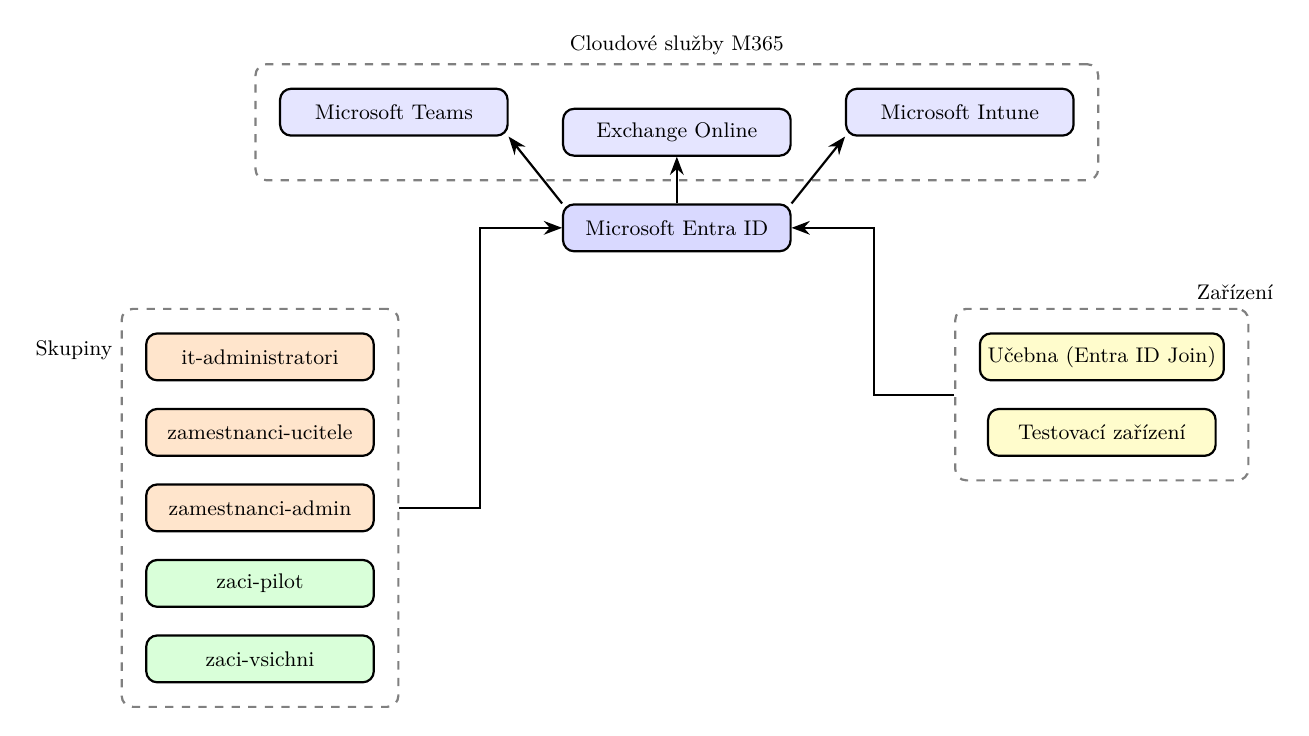
\begin{tikzpicture}[
    scale=0.85,
    transform shape,
    node distance=1.0cm and 1.2cm,
    box/.style={rectangle, rounded corners, draw=black, thick,
                minimum width=3.4cm, minimum height=0.7cm,
                text centered, font=\small},
    groupbox/.style={rectangle, rounded corners, draw=gray, dashed,
                thick, inner sep=0.3cm},
    arrow/.style={-{Stealth}, thick},
]

% Entra ID centrum
\node[box, fill=blue!15] (entra) {Microsoft Entra ID};

% Skupiny vlevo
\node[box, fill=orange!20, below left=1.2cm and 2.8cm of entra] (itadmin)
    {\texttt{it-administratori}};
\node[box, fill=orange!20, below=0.4cm of itadmin] (ucitele)
    {\texttt{zamestnanci-ucitele}};
\node[box, fill=orange!20, below=0.4cm of ucitele] (admin)
    {\texttt{zamestnanci-admin}};
\node[box, fill=green!15, below=0.4cm of admin] (pilot)
    {\texttt{zaci-pilot}};
\node[box, fill=green!15, below=0.4cm of pilot] (zaci)
    {\texttt{zaci-vsichni}};

% Skupiny rámeček
\begin{pgfonlayer}{background}
\node[groupbox, fit=(itadmin)(zaci),
    label=above left:{\small Skupiny}] (skupiny_box) {};
\end{pgfonlayer}

% Zařízení vpravo
\node[box, fill=yellow!20, below right=1.2cm and 2.8cm of entra] (ucebna)
    {U\v{c}ebna (Entra ID Join)};
\node[box, fill=yellow!20, below=0.4cm of ucebna] (pilot_pc)
    {Testovac\'{i} za\v{r}\'{i}zen\'{i}};

% Zařízení rámeček
\begin{pgfonlayer}{background}
\node[groupbox, fit=(ucebna)(pilot_pc),
    label=above right:{\small Za\v{r}\'{i}zen\'{i}}] (zarizeni_box) {};
\end{pgfonlayer}

% Cloudové služby nahoře
\node[box, fill=blue!10, above left=1.0cm and 0.8cm of entra] (teams)
    {Microsoft Teams};
\node[box, fill=blue!10, above=0.7cm of entra] (exchange)
    {Exchange Online};
\node[box, fill=blue!10, above right=1.0cm and 0.8cm of entra] (intune)
    {Microsoft Intune};

% Cloudové služby rámeček
\begin{pgfonlayer}{background}
\node[groupbox, fit=(teams)(exchange)(intune),
    label=above:{\small Cloudov\'{e} slu\v{z}by M365}] {};
\end{pgfonlayer}

% Šipky
\draw[arrow] (skupiny_box.east) -- ++(1.2,0) |- (entra.west);
\draw[arrow] (zarizeni_box.west) -- ++(-1.2,0) |- (entra.east);
\draw[arrow] (entra.north west) -- (teams.south east);
\draw[arrow] (entra.north) -- (exchange.south);
\draw[arrow] (entra.north east) -- (intune.south west);

\end{tikzpicture}
\shorthandon{-}
\caption{Navr\v{z}en\'{a} architektura spr\'{a}vy identit v~Microsoft Entra ID}
\label{fig:architektura}
\end{figure}

Uživatelské účty budou organizovány do bezpečnostních skupin podle role 
uživatele ve škole. Navržená skupinová struktura je uvedena v~tabulce 
\ref{tab:skupiny}.

\begin{table}[h]
\centering
\caption{Navržená struktura skupin v~Microsoft Entra ID}
\label{tab:skupiny}
\begin{tabular}{|p{4.5cm}|p{8.5cm}|}
\hline
\textbf{Název skupiny} & \textbf{Účel} \\
\hline
\texttt{zaci-vsichni} & Všichni žáci tenanta; určena pro aplikaci globálních politik \\
\hline
\texttt{zaci-pilot} & Pilotní skupina testovacích účtů; cíl politik při pilotním ověření \\
\hline
\texttt{zamestnanci-ucitele} & Pedagogičtí pracovníci \\
\hline
\texttt{zamestnanci-admin} & Nepedagogický a~administrativní personál \\
\hline
\texttt{it-administratori} & IT správci; cílová skupina pro MFA a~politiky podmíněného přístupu \\
\hline
\end{tabular}
\end{table}

\subsection{Připojení zařízení do Entra ID}

Počítače určené pro výuku budou připojeny do Microsoft Entra ID prostřednictvím 
funkce Entra ID Join. Toto připojení umožňuje centrální správu zařízení 
prostřednictvím Microsoft Intune, vynucování bezpečnostních politik a~přihlášení 
uživatelů pomocí jejich cloudové identity bez nutnosti lokálního účtu. 
Předpokladem pro Entra ID Join je provoz operačního systému Windows 10 nebo 
Windows~11 v~edici Pro nebo Enterprise. Testovací zařízení dostupná pro pilotní 
nasazení jsou vybavena edicí Windows~11 Home, která tuto funkci nepodporuje. 
Před samotným připojením do Entra ID bude proto nutné provést upgrade na edici 
Windows~11 Pro Education, na níž má škola nárok v~rámci licencí 
Microsoft~365 Education~A3 bez dodatečných nákladů.

Zařízení provozovaná v~rámci pronájmu od externího poskytovatele jsou z~rozsahu 
navrhované implementace vyloučena, neboť jejich správa podléhá smluvním 
podmínkám pronájmu a~připojení do školního tenanta by vyžadovalo souhlas 
pronajímatele.

\subsection{Vícefaktorové ověřování a podmíněný přístup}

V~rámci navrženého řešení bude vícefaktorové ověřování povinně zavedeno pro 
skupinu \texttt{it-\allowbreak administratori}. Tato skupina představuje nejvyšší rizikový 
profil z~hlediska dopadu případné kompromitace účtu, neboť její členové 
disponují globálními administrátorskými oprávněními v~rámci tenanta. 
Jako primární metoda MFA bude použita aplikace Microsoft Authenticator. 
Vynucení MFA bude realizováno prostřednictvím politiky podmíněného přístupu 
(Conditional Access), která bude cílit na skupinu \texttt{it-\allowbreak administratori}
a~vyžadovat splnění MFA při každém přihlášení ke cloudovým službám školy.

Rozšíření MFA na skupinu pedagogických pracovníků je plánováno jako součást plného produkčního nasazení po skončení školního roku. Toto odložení vychází z~provozních omezení popsaných výše a~není opomenutím dílčího cíle práce.

\section{Návrh bezpečnostních politik a správy zařízení}

Správa zařízení a~vynucování bezpečnostních politik bude realizováno 
prostřednictvím Microsoft Intune, cloudové služby pro správu koncových 
zařízení zahrnuté v~licencích Microsoft~365 Education~A3. Vzhledem k~tomu, 
že navrhovaná infrastruktura je postavena výhradně na cloudové adresářové 
službě Microsoft Entra ID bez lokálního Active Directory, nelze využít 
tradiční skupinové politiky (GPO, z angl. Group Policy Objects), které vyžadují připojení k~doméně. 
Intune v~kombinaci s~nástrojem Settings Catalog představuje funkční 
ekvivalent GPO v~cloudovém prostředí a~umožňuje centrální konfiguraci 
zařízení, vynucování bezpečnostních nastavení a~vzdálenou správu 
bez nutnosti fyzického přístupu k~zařízení.

\subsection{Správa zařízení prostřednictvím Microsoft Intune}

Po připojení zařízení do Microsoft Entra ID prostřednictvím Entra ID Join 
budou zařízení automaticky zaregistrována v~Microsoft Intune. Tato 
registrace umožní aplikovat na zařízení konfigurační profily a~bezpečnostní 
politiky centrálně spravované IT administrátorem bez nutnosti lokálního 
zásahu na každém stroji.

Pro žákovské stanice v~počítačové učebně bude prostřednictvím Intune 
aplikována sada politik zahrnující následující oblasti:

\begin{itemize}
    \item \textbf{Windows Security Baseline:} Předdefinovaná sada 
    bezpečnostních nastavení doporučená společností Microsoft, zahrnující 
    konfiguraci Windows Defenderu, firewallu a~základních systémových 
    nastavení.
    \item \textbf{Restrikce instalace softwaru:} Uživatelé bez 
    administrátorských oprávnění nebudou moci instalovat aplikace 
    bez schválení IT administrátorem.
    \item \textbf{Konfigurace prohlížeče:} Prostřednictvím 
    konfiguračního profilu pro Microsoft Edge budou nastavena omezení 
    přístupu k~nevhodným kategoriím obsahu a~zakázána možnost ukládání 
    hesel v~prohlížeči.
    \item \textbf{Automatické zamykání obrazovky:} Zařízení se 
    automaticky zamkne po definované době nečinnosti.
\end{itemize}

\subsection{Politika hesel}

Správně nastavená politika hesel tvoří základ ochrany uživatelských účtů. 
Bez centrálního vynucení požadavků na hesla nelze zaručit, že uživatelé 
nezvolí snadno uhodnutelná nebo již kompromitovaná hesla, což platí 
zejména ve školním prostředí, kde není možné spoléhat na bezpečnostní 
povědomí všech uživatelů.

V~rámci Microsoft Entra ID bude nakonfigurována funkce Password Protection, 
která blokuje použití slabých a~kompromitovaných hesel. Funkce pracuje 
se dvěma seznamy zakázaných hesel: globálním seznamem spravovaným 
společností Microsoft, který obsahuje hesla z~veřejně dostupných databází 
uniklých přihlašovacích údajů, a~vlastním seznamem organizace, do nějž 
lze doplnit výrazy specifické pro školní prostředí, například názvy školy 
nebo obecná slova jako \textit{škola} či \textit{heslo}. Minimální délka 
hesla bude nastavena v~souladu s~doporučeními NIST, která upřednostňují 
délku hesla před složitostí a~nedoporučují vynucovat pravidelné změny 
hesla bez konkrétního důvodu~\cite{NIST_SP800634}. Funkce Password 
Protection je součástí Entra ID Premium P1, jež je školám dostupná 
v~rámci licence Microsoft~365 Education~A3~\cite{MicrosoftEntra2025}.

\subsection{Šifrování disků pomocí BitLocker}

Součástí návrhu je zavedení šifrování disků prostřednictvím technologie 
BitLocker na všech zařízeních připojených do Entra ID. Šifrování disku 
zajišťuje ochranu dat v~případě fyzické ztráty nebo odcizení zařízení, 
přičemž bez znalosti šifrovacího klíče není možné získat přístup k~datům 
uloženým na disku. Správa šifrovacích klíčů bude realizována centrálně 
prostřednictvím Microsoft Intune, kde jsou klíče pro obnovu uloženy 
v~rámci záznamu každého zařízení. IT administrátor tak má možnost 
v~případě potřeby klíč dohledat bez nutnosti fyzického přístupu k~zařízení.

BitLocker bude aktivován automaticky prostřednictvím konfiguračního 
profilu Intune po úspěšném připojení zařízení do Entra ID. Předpokladem 
je přítomnost čipu TPM (Trusted Platform Module) ve verzi 2.0, 
který je vyžadován pro uložení šifrovacího klíče. Dostupnost čipu TPM 
bude ověřena v~rámci pilotního nasazení popsaného v~kapitole~5.

\subsection{Shrnutí navržených opatření}

Navržená sada bezpečnostních opatření reaguje přímo na nedostatky 
identifikované v~analýze současného stavu. Přechod na individuální 
cloudové identity v~kombinaci s~centrální správou zařízení prostřednictvím 
Intune zajistí auditní stopu, umožní vynucovat jednotné bezpečnostní 
politiky napříč zařízeními a~sníží administrativní zátěž spojenou 
se správou lokálních účtů. Implementace navržených opatření je 
předmětem následující kapitoly.

\chapter{Pilotní nasazení a~implementace bezpečnostních opatření}

Tato kapitola popisuje průběh pilotního nasazení navržené architektury správy 
identit a~bezpečnostních opatření na ZŠ Vinařská. Implementace byla provedena 
v~prostředí Microsoft~365 Education a~Microsoft Intune s~využitím globálních 
administrátorských oprávnění IT administrátora školy. Veškeré kroky byly 
dokumentovány formou screenshotů z~administrátorských portálů.

Vzhledem k~tomu, že počítačové stanice jsou v~době zpracování této práce 
aktivně využívány při výuce, nebylo možné provést plné produkční nasazení 
bez narušení provozu školy. Pilotní nasazení bylo proto realizováno 
na jednom testovacím zařízení vyřazeném z~produkčního provozu, označeném 
jako NTB001, a~na jednom testovacím uživatelském účtu. Na základě dohody 
s~vedením školy je plné produkční nasazení naplánováno na období letních 
prázdnin 2026, kdy bude možné připojit všechna zařízení do Microsoft Entra ID 
a~provést migraci uživatelských účtů bez dopadu na výuku.

\section{Vytvoření skupin v~Microsoft Entra ID}

Prvním krokem implementace bylo vytvoření bezpečnostních skupin v~Microsoft 
Entra ID podle struktury navržené v~kapitole~4. Skupiny byly vytvořeny prostřednictvím portálu \url{entra.microsoft.com} s~využitím globálního 
administrátorského účtu. Každá skupina byla nakonfigurována jako skupina 
typu Zabezpečení s~přiřazeným typem členství.

\begin{figure}[H]
\centering

\includegraphics[width=0.8\textwidth]{Práce/Obrázky/obrázek_2026-04-28_220306947.png}
\caption{Přehled vytvořených bezpečnostních skupin v~Microsoft Entra ID}
\label{fig:skupiny-prehled}
\end{figure}

Celkem bylo vytvořeno pět skupin odpovídajících navrženým rolím uživatelů. 
Do skupiny \texttt{it-\allowbreak administratori} byl přidán účet IT administrátora 
školy, který slouží jako cílová skupina pro politiku vícefaktorového ověřování.

\section{Konfigurace vícefaktorového ověřování}

Po vytvoření skupin byla nakonfigurována politika podmíněného přístupu 
vynucující vícefaktorové ověřování pro skupinu \texttt{it-administratori}. 
Politika byla vytvořena v~sekci Conditional Access portálu Microsoft Entra ID 
pod názvem \texttt{MFA-it-administratori}. Politika cílí na skupinu 
\texttt{it-administratori}, zahrnuje všechny cloudové aplikace a~jako 
ovládací prvek přístupu vyžaduje vícefaktorové ověřování. Politika byla 
aktivována v~režimu Zapnuto.

\begin{figure}[H]
\centering

\includegraphics[width=0.8\textwidth]{Práce/Obrázky/obrázek_2026-04-28_220428058.png}
\caption{Přehled politik podmíněného přístupu včetně aktivní politiky 
\texttt{MFA-it-administratori}}
\label{fig:ca-prehled}
\end{figure}

Funkčnost politiky byla ověřena praktickým testem. Po odhlášení 
a~opětovném přihlášení administrátorského účtu systém vyzval uživatele 
k~ověření prostřednictvím aplikace Microsoft Authenticator s~číselným 
kódem (number matching). Tím bylo potvrzeno správné fungování politiky 
podmíněného přístupu.

\begin{figure}[H]
\centering

\includegraphics[width=0.5\textwidth]{Práce/Obrázky/obrázek_2026-04-28_220437277.png}
\caption{Výzva k~ověření prostřednictvím aplikace Microsoft Authenticator}
\label{fig:mfa-vyzva}
\end{figure}

\section{Příprava testovacího zařízení}

Testovací zařízení bylo vybaveno operačním systémem Windows~11 Home, 
který nepodporuje připojení do Microsoft Entra ID. Před samotným 
připojením bylo proto nutné provést upgrade na edici Windows~11 
Pro Education. Vzhledem k~tomu, že zařízení bylo vybaveno OEM (z angl. Original Equipment Manufacturer) digitální licencí vázanou na hardware, nebylo možné použít standardní postup 
změny edice pomocí kódu Product Key ani prostřednictvím nástroje DISM (z angl. Deployment Image Servicing and Management). 
Upgrade byl proto proveden čistou instalací systému Windows~11 
Pro Education z~bootovacího USB média vytvořeného nástrojem Rufus, open-source aplikací pro vytváření bootovacích USB médií.

Po dokončení instalace bylo zařízení při prvotním nastavení připojeno 
do Microsoft Entra ID prostřednictvím volby Nastavit pro práci nebo 
školu. Přihlášení bylo provedeno administrátorským účtem 
\texttt{bao.kieuquang@zsvinarska.cz}.

\begin{figure}[H]
\centering

\includegraphics[width=0.8\textwidth]{Práce/Obrázky/obrázek_2026-04-28_220457404.png}
\caption{Potvrzení připojení zařízení do Microsoft Entra ID 
v~nastavení systému Windows}
\label{fig:entraid-join}
\end{figure}

Úspěšné připojení zařízení bylo ověřeno v~portálu Microsoft Entra ID, 
kde se zařízení NTB001 zobrazilo s~typem připojení Microsoft Entra Join, 
stavem Povoleno a~automaticky přiřazenou správou prostřednictvím 
Microsoft Intune.

\begin{figure}[H]
\centering

\includegraphics[width=0.8\textwidth]{Práce/Obrázky/obrázek_2026-04-28_220506697.png}
\caption{Zařízení NTB001 zaregistrované v~Microsoft Entra ID 
s~automatickou registrací v~Microsoft Intune}
\label{fig:ntb001-entra}
\end{figure}

\section{Nasazení bezpečnostních politik prostřednictvím Microsoft Intune}

Po úspěšném připojení zařízení do Entra ID byly v~Microsoft Intune 
vytvořeny a~přiřazeny bezpečnostní politiky pro skupinu \texttt{zaci-pilot}.

\subsection{Windows Security Baseline}

Jako první byla nasazena předdefinovaná sada bezpečnostních nastavení 
Windows Security Baseline ve verzi 25H2. Tato baseline zahrnuje 
doporučená nastavení Windows Defenderu, firewallu a~dalších systémových 
komponent dle doporučení společnosti Microsoft. Politika byla přiřazena 
skupině \texttt{zaci-pilot} a~nazvána \texttt{Windows-Security-Baseline-Zaci}.

\subsection{Restrikce instalace softwaru}

Druhá politika byla vytvořena prostřednictvím nástroje Settings Catalog 
a~nakonfigurována tak, aby uživatelům bez administrátorských oprávnění 
znemožnila instalaci neautorizovaných aplikací. Konkrétně bylo nastaveno 
\textit{Disable Windows Installer} na hodnotu \textit{For non-managed 
applications only}, čímž je instalace povolena pouze pro aplikace 
nasazené prostřednictvím Intune.

\subsection{Konfigurace prohlížeče Microsoft Edge}

Třetí politika nakonfigurovala bezpečnostní nastavení prohlížeče 
Microsoft Edge. Byla aktivována funkce \textit{Enforce Bing SafeSearch} 
v~režimu středních omezení, která filtruje nevhodný obsah ve výsledcích 
vyhledávání. Dále bylo zakázáno ukládání přístupových klíčů 
v~integrovaném správci hesel prohlížeče.

\subsection{Šifrování disků pomocí BitLocker}

Poslední politika nakonfigurovala šifrování systémového disku 
prostřednictvím technologie BitLocker. Byl zvolen šifrovací algoritmus 
AES-CBC 128-bit pro systémový disk a~AES-CBC 128-bit pro vyměnitelná 
média. Typ šifrování byl nastaven na úplné šifrování disku 
(Full encryption). Obnovovací klíče jsou automaticky ukládány 
do Microsoft Entra ID, přičemž aktivace BitLockeru je podmíněna 
úspěšným uložením klíče.

\section{Ověření synchronizace politik}

Pro účely pilotního testování byl vytvořen testovací uživatelský účet 
\texttt{test.zak@zsvinarska.cz} reprezentující žákovský účet. Tento 
účet byl přidán do skupiny \texttt{zaci-pilot} spolu se zařízením NTB001. 
Po přihlášení testovacího účtu na zařízení NTB001 a~provedení synchronizace 
bylo v~portálu Microsoft Intune potvrzeno úspěšné aplikování všech 
nasazených politik. Konkrétně byly jako úspěšné označeny všechny čtyři nasazené politiky pro skupinu \texttt{zaci-pilot}: Windows Security Baseline, politika BitLockeru, konfigurace prohlížeče Edge a~restrikce instalace softwaru.

\begin{figure}[H]
\centering

\includegraphics[width=0.8\textwidth]{Práce/Obrázky/obrázek_2026-04-28_225128604.png}
\caption{Stav aplikovaných konfiguračních politik na zařízení NTB001 
v~Microsoft Intune po synchronizaci}
\label{fig:intune-sync}
\end{figure}

\begin{figure}[H]
\centering

\includegraphics[width=0.8\textwidth]{Práce/Obrázky/obrázek_2026-04-28_221019872.png}
\caption{Členové skupiny \texttt{zaci-pilot} zahrnující zařízení NTB001 
a~testovací uživatelský účet}
\label{fig:zaci-pilot-clenove}
\end{figure}

Pilotní nasazení potvrdilo funkčnost navrženého řešení v~reálném prostředí 
školního tenanta Microsoft~365. Ověřená konfigurace tvoří základ pro plné 
produkční nasazení, v~jehož rámci budou do Microsoft Entra ID připojena 
všechna zařízení počítačové učebny a~provedena migrace všech žákovských 
a~pedagogických účtů na individuální cloudové identity.

\chapter{Scénář zapůjčeného notebooku, pilotní nasazení a~vyhodnocení}

\section{Scénář zapůjčeného notebooku}

Součástí navržené architektury je rovněž scénář zapůjčení školního notebooku 
žákovi domů. Tento scénář je relevantní zejména v~kontextu distanční výuky 
nebo individuální práce žáků mimo školní prostředí. Proces zapůjčení 
a~správy zařízení je popsán níže jako teoretický model, jehož plné ověření 
v~praxi je plánováno po produkčním nasazení v~průběhu letních prázdnin 2026.

\subsection{Proces předání zařízení}

Před zapůjčením zařízení žákovi je nutné splnit administrativní 
a~technické předpoklady. Po administrativní stránce je zapůjčení 
podmíněno podpisem předávacího protokolu žákem a~jeho zákonným zástupcem, 
čímž je jasně stanovena odpovědnost za svěřené zařízení. Po technické 
stránce musí být zařízení připojeno do Microsoft Entra ID a~zaregistrováno 
v~Microsoft Intune, přičemž na něj musí být aplikovány příslušné 
konfigurační profily a~bezpečnostní politiky.

\subsection{První přihlášení a~aplikované politiky}

Po fyzickém převzetí zařízení se žák přihlásí svým individuálním školním 
účtem ve formátu \texttt{jmeno.prijmeni@zsvinarska.cz}. Díky připojení 
zařízení do Entra ID probíhá přihlášení cloudovou identitou bez nutnosti 
lokálního účtu. Po přihlášení jsou automaticky aplikovány všechny politiky 
přiřazené skupině \texttt{zaci-vsichni}, včetně restrikcí instalace 
softwaru, konfigurace prohlížeče a~šifrování disku prostřednictvím 
BitLockeru. Žákova data jsou prostřednictvím služby OneDrive automaticky 
zálohována do cloudu, čímž je zajištěna jejich dostupnost i~z~jiných 
zařízení a~ochrana před ztrátou.

\subsection{Řešení incidentů}

Nejzávažnějším incidentem v~kontextu zapůjčeného zařízení je jeho ztráta 
nebo krádež. Díky šifrování disku technologií BitLocker jsou data na 
zařízení chráněna před neoprávněným přístupem i~v~případě fyzického 
odcizení. IT administrátor má prostřednictvím Microsoft Intune možnost vzdáleně provést vymazání zařízení (remote wipe), tedy obnovení do továrního nastavení. 
Tím je zabráněno zneužití školních dat nebo 
přihlašovacích údajů. Veškerá žákova data jsou přitom zachována 
v~cloudovém úložišti OneDrive a~nejsou výmazem zařízení dotčena.

\section{Pilotní nasazení a~zpětná vazba}

Navržené řešení bylo v~rámci pilotního nasazení popsaného v~kapitole~5 
ověřeno na testovacím zařízení NTB001 s~testovacím uživatelským účtem. 
Nad rámec technického testování bylo řešení prezentováno žákům sedmého 
a~osmého ročníku ZŠ Vinařská. Žáci devátého ročníku do prezentace 
zahrnuti nebyli, neboť se blíží jejich odchod ze školy a~zavedení 
systému by se jich v~praxi nedotklo. Mladší žáci prvního stupně by 
naopak navrhovanému řešení nemuseli plně porozumět, proto byli 
z~prezentace rovněž vynecháni.

Prezentace proběhla formou živé ukázky pro přibližně 60 žáků, přičemž reakce byly převážně pozitivní. 
Největší zájem vzbudila možnost individuálního pracovního prostoru, žáci ocenili 
zejména skutečnost, že jejich práce bude chráněna před neoprávněnými 
zásahy ostatních uživatelů a~že budou mít přístup ke svým souborům 
z~libovolné stanice v~učebně. Tato zpětná vazba potvrzuje že přechod 
od sdílených lokálních účtů k~individuálním cloudovým identitám odpovídá 
reálným potřebám uživatelů.

\section{Metriky úspěchu}

Úspěšnost pilotního nasazení byla hodnocena na základě následujících 
kritérií:

\begin{itemize}
    \item \textbf{Technická funkčnost:} Všechny nasazené politiky 
    (\texttt{Windows-Security-Baseline-Zaci}, 
    \texttt{Restrikce-\allowbreak Instalace-\allowbreak Softwaru-\allowbreak Zaci}, 
    \texttt{Konfigurace-\allowbreak Edge-\allowbreak Zaci}, 
    \texttt{BitLocker-\allowbreak Zaci}) byly po synchronizaci 
    označeny stavem Úspěšné v~portálu Microsoft Intune.
    \item \textbf{Funkčnost MFA:} Politika podmíněného přístupu 
    \texttt{MFA-it-administratori} byla úspěšně ověřena praktickým 
    testem přihlášení s~výzvou Microsoft Authenticator.
    \item \textbf{Entra ID Join:} Testovací zařízení NTB001 bylo 
    úspěšně připojeno do Microsoft Entra ID a~automaticky 
    zaregistrováno v~Microsoft Intune.
    \item \textbf{Zpětná vazba uživatelů:} Prezentace řešení žákům 
    sedmého a~osmého ročníku přinesla pozitivní ohlasy, zejména 
    v~oblasti ochrany individuálních dat a~přístupu ke školním 
    službám z~libovolného zařízení.
\end{itemize}

\section{Implementační plán}

Realizace navrhovaného řešení probíhá ve dvou fázích. První fáze 
zahrnovala pilotní nasazení ověřené v~rámci této práce, druhá fáze 
představuje plné produkční nasazení plánované na období letních 
prázdnin 2026, kdy nebude docházet k~narušení výuky.

\begin{table}[h]
\centering
\caption{Časová osa implementace}
\label{tab:implementacni-plan}
\begin{tabular}{|p{3cm}|p{3cm}|p{7cm}|}
\hline
\textbf{Fáze} & \textbf{Období} & \textbf{Obsah} \\
\hline
Pilotní nasazení & Duben 2026 & 
Vytvoření skupin v~Entra ID, konfigurace MFA pro IT administrátory, 
připojení testovacího zařízení NTB001 do Entra ID, nasazení 
bezpečnostních politik prostřednictvím Intune, ověření synchronizace. \\
\hline
Produkční nasazení & Červenec--srpen 2026 & 
Připojení všech zařízení počítačové učebny do Entra ID, migrace 
žákovských a~pedagogických účtů na individuální cloudové identity, 
rozšíření MFA na skupinu pedagogických pracovníků, zapojení 
zapůjčených notebooků do správy prostřednictvím Intune. \\
\hline
Školení uživatelů & Září 2026 & 
Seznámení pedagogických pracovníků s~novým způsobem přihlašování 
a~MFA, základní instrukce pro žáky k~používání individuálních účtů 
a~cloudového úložiště OneDrive. \\
\hline
\end{tabular}
\end{table}

\section{Vyhodnocení přínosů a~rizik}

\subsection{Přínosy navrženého řešení}

Navržená a~pilotně ověřená architektura přináší ZŠ Vinařská několik 
konkrétních přínosů. Přechod od sdílených lokálních účtů k~individuálním 
cloudovým identitám zajišťuje jednoznačnou identifikaci každého uživatele 
a~vytváří auditní stopu, která byla v~předchozím stavu zcela absentující. 
Tím škola získává schopnost prokázat soulad se zásadami odpovědnosti 
a~prokazatelnosti vyžadovanými nařízením GDPR.

Centrální správa zařízení prostřednictvím Microsoft Intune umožňuje 
IT administrátorovi vynucovat jednotné bezpečnostní politiky napříč 
všemi zařízeními bez nutnosti fyzického přístupu ke každému stroji. 
Šifrování disků technologií BitLocker s~centrálním uložením obnovovacích 
klíčů v~Entra ID pak zajišťuje ochranu dat i~při fyzické ztrátě zařízení.

Z~pohledu žáků a~pedagogů přináší řešení přístup k~individuálnímu 
pracovnímu prostoru dostupnému z~libovolné školní stanice, ochranu 
vlastních dat před neoprávněnými zásahy a~možnost bezpečné práce 
se školními službami sady Microsoft~365.

\subsection{Identifikovaná rizika a~doporučení}

V~průběhu pilotního nasazení a~analýzy prostředí byla identifikována 
následující rizika a~odpovídající doporučení pro jejich zmírnění:

\begin{itemize}
    \item \textbf{Připojení soukromých zařízení do školního tenanta:} 
    Žák může při domácím nastavení počítače připojit soukromé zařízení 
    do školního tenanta, čímž by na něj byly aplikovány školní politiky. 
    Doporučuje se omezit maximální počet zařízení na uživatele 
    v~nastavení Entra ID na hodnotu odpovídající počtu zapůjčených 
    školních zařízení.
    \item \textbf{Správa hesel žáků:} Žáci základní školy, zejména 
    mladšího věku, nejsou schopni samostatně obnovit zapomenuté heslo. 
    Aktuálním řešením je centrální reset hesla IT administrátorem. 
    Pro starší žáky druhého stupně a~pedagogické pracovníky je 
    doporučeno zvážit zavedení služby SSPR (z angl. Self-Service Password Reset, samoobslužné obnovení hesla), která umožní samostatnou obnovu hesla prostřednictvím 
    ověřovací metody.
    \item \textbf{Pronajatá zařízení:} Část notebooků je provozována 
    v~rámci pronájmu od externího poskytovatele. Tato zařízení jsou 
    z~rozsahu implementace vyloučena, neboť jejich připojení do školního 
    tenanta by vyžadovalo souhlas pronajímatele. Doporučuje se tuto 
    otázku řešit při případné obnově smlouvy o~pronájmu.
    \item \textbf{Rozšíření MFA:} V~pilotním nasazení je MFA zavedeno 
    pouze pro skupinu IT administrátorů. Po úspěšném produkčním 
    nasazení je doporučeno rozšířit povinné MFA na skupinu 
    pedagogických pracovníků.
    \item \textbf{Správa tabletů:} Škola disponuje tablety, které 
    nejsou v~současnosti spravovány prostřednictvím Intune. 
    Microsoft Intune podporuje správu zařízení s~operačními systémy 
    Android i~iOS, a~jejich zapojení do centrální správy je proto 
    doporučeno jako součást produkčního nasazení po ověření 
    kompatibility a~případném vyjednání souhlasu poskytovatele pronájmu.
\end{itemize}

\chapter{Závěr}
Práce se zabývá přechodem ze sdílených lokálních účtů na individuální cloudové identity na ZŠ Vinařská. Analýza odhalila konkrétní nedostatky v oblasti správy identit a přístupů. Chybějící vícefaktorové ověřování, nekonfigurovaný podmíněný přístup a absence centrální správy zařízení představovaly bezprostřední bezpečnostní rizika i překážku v plnění povinností vyplývajících z nařízení GDPR.

Na základě provedené analýzy byl navržen architekturní model postavený na cloudové adresářové službě Microsoft Entra ID. Model zahrnuje strukturu bezpečnostních skupin, konvenci pojmenování účtů, nasazení vícefaktorového ověřování a podmíněného přístupu, politiku hesel a správu zařízení prostřednictvím Microsoft Intune včetně šifrování disků technologií BitLocker.

Navržené řešení bylo ověřeno pilotním nasazením na testovacím zařízení NTB001, které bylo připojeno do Microsoft Entra ID a zaregistrováno v Microsoft Intune. Na zařízení byly úspěšně nasazeny čtyři bezpečnostní politiky a ověřena funkčnost vícefaktorového ověřování. Navržené řešení bylo prezentováno formou živé ukázky přibližně 60 žákům sedmého a osmého ročníku, přičemž reakce byly převážně pozitivní. Implementační plán stanovuje plné produkční nasazení na období letních prázdnin 2026.

\sloppy
\printbibliography[title=Seznam použitých zdrojů]

\appendix

\chapter{Externí přílohy\label{sec:ep}}

Externí přílohy této bakalářské práce jsou umístěny na adrese:\\ \url{https://github.com/ChaoZavitkar/KI_UJEP_thesis}.

Repozitář obsahuje zdrojové soubory potřebné pro překlad dokumentu
a konfigurační dokumentaci určenou pro správce a vedení školy.

\begin{longtable}{ll}
\hline
main\_text.tex & zdrojový kód práce v \LaTeX{}u \\
thesis.bib & bibliografická databáze \\
kitheses.cls & definice třídy dokumentů \\
LOGO\_PRF\_CZ\_RGB\_standard.jpg & logo fakulty s českým textem \\
Konfiguracni\_dokumentace.pdf & konfigurační dokumentace pro správce školy \\
\hline
\end{longtable}

Všechny soubory jsou potřeba pro překlad dokumentu. Logo stačí
v~české jazykové verzi. Konfigurační dokumentace je samostatný dokument
určený pro IT administrátora a vedení školy, popisující správu uživatelů,
politiky Intune, MFA a postup při incidentech se zapůjčenými zařízeními.

\end{document}

